\documentclass[10pt,twocolumn]{article}
% Shared two-column preamble for the three research papers.
% Use with: \documentclass[10pt,twocolumn]{article}
% Then in main.tex: % Shared two-column preamble for the three research papers.
% Use with: \documentclass[10pt,twocolumn]{article}
% Then in main.tex: % Shared two-column preamble for the three research papers.
% Use with: \documentclass[10pt,twocolumn]{article}
% Then in main.tex: \input{../../shared/latex/twocolumn_preamble.tex}

\usepackage[margin=0.75in]{geometry}
\usepackage[utf8]{inputenc}
\usepackage[T1]{fontenc}
\usepackage{lmodern}
\usepackage{microtype}
\usepackage{amsmath,amssymb,amsthm}
\usepackage{graphicx}
\usepackage{booktabs}
\usepackage{caption}
\usepackage{subcaption}
\usepackage{hyperref}
\usepackage{url}
\usepackage{xcolor}
\usepackage{algorithm}
\usepackage{algorithmic}
\usepackage{multirow}
\usepackage{titlesec}
\usepackage{authblk}

\hypersetup{colorlinks=true,linkcolor=blue!50!black,citecolor=blue!50!black,urlcolor=blue!50!black}

\titleformat{\section}{\normalfont\large\bfseries}{\thesection}{0.6em}{}
\titleformat{\subsection}{\normalfont\bfseries}{\thesubsection}{0.5em}{}

\captionsetup{font=small,labelfont=bf,skip=4pt}
\setlength{\columnsep}{0.25in}
\setlength{\parskip}{2pt}

\newtheorem{theorem}{Theorem}
\newtheorem{proposition}[theorem]{Proposition}
\newtheorem{definition}[theorem]{Definition}


\usepackage[margin=0.75in]{geometry}
\usepackage[utf8]{inputenc}
\usepackage[T1]{fontenc}
\usepackage{lmodern}
\usepackage{microtype}
\usepackage{amsmath,amssymb,amsthm}
\usepackage{graphicx}
\usepackage{booktabs}
\usepackage{caption}
\usepackage{subcaption}
\usepackage{hyperref}
\usepackage{url}
\usepackage{xcolor}
\usepackage{algorithm}
\usepackage{algorithmic}
\usepackage{multirow}
\usepackage{titlesec}
\usepackage{authblk}

\hypersetup{colorlinks=true,linkcolor=blue!50!black,citecolor=blue!50!black,urlcolor=blue!50!black}

\titleformat{\section}{\normalfont\large\bfseries}{\thesection}{0.6em}{}
\titleformat{\subsection}{\normalfont\bfseries}{\thesubsection}{0.5em}{}

\captionsetup{font=small,labelfont=bf,skip=4pt}
\setlength{\columnsep}{0.25in}
\setlength{\parskip}{2pt}

\newtheorem{theorem}{Theorem}
\newtheorem{proposition}[theorem]{Proposition}
\newtheorem{definition}[theorem]{Definition}


\usepackage[margin=0.75in]{geometry}
\usepackage[utf8]{inputenc}
\usepackage[T1]{fontenc}
\usepackage{lmodern}
\usepackage{microtype}
\usepackage{amsmath,amssymb,amsthm}
\usepackage{graphicx}
\usepackage{booktabs}
\usepackage{caption}
\usepackage{subcaption}
\usepackage{hyperref}
\usepackage{url}
\usepackage{xcolor}
\usepackage{algorithm}
\usepackage{algorithmic}
\usepackage{multirow}
\usepackage{titlesec}
\usepackage{authblk}

\hypersetup{colorlinks=true,linkcolor=blue!50!black,citecolor=blue!50!black,urlcolor=blue!50!black}

\titleformat{\section}{\normalfont\large\bfseries}{\thesection}{0.6em}{}
\titleformat{\subsection}{\normalfont\bfseries}{\thesubsection}{0.5em}{}

\captionsetup{font=small,labelfont=bf,skip=4pt}
\setlength{\columnsep}{0.25in}
\setlength{\parskip}{2pt}

\newtheorem{theorem}{Theorem}
\newtheorem{proposition}[theorem]{Proposition}
\newtheorem{definition}[theorem]{Definition}

\newcommand{\SpeNGraphs}{96}
\newcommand{\SpeRatioMin}{4.0}
\newcommand{\SpeRatioMax}{123}
\newcommand{\SpeRatioAllAboveOne}{all}
\newcommand{\SpeCurlHarmMin}{0.80}
\newcommand{\SpeCurlHarmMax}{1.71}
\newcommand{\SpeCurlHarmMean}{1.02}
\newcommand{\SpeScalarCycMax}{3\times10^{-16}}
\newcommand{\SpeRatioDense}{63}
\newcommand{\SpeRatioSparse}{13.8}
\newcommand{\SpeRatioDepthOne}{34.6}
\newcommand{\SpeRatioDepthTwo}{17.0}
\newcommand{\SpeRatioLowD}{48.4}
\newcommand{\SpeRatioHighD}{26.2}
\newcommand{\SpeLowD}{2}
\newcommand{\SpeHighD}{32}
\newcommand{\SpeTopTenGradMass}{99}
\newcommand{\SpeCanonN}{30}
\newcommand{\SpeCanonE}{109}
\newcommand{\SpeCanonGradDim}{29}
\newcommand{\SpeCanonCurlDim}{51}
\newcommand{\SpeCanonHarmDim}{29}
\newcommand{\SpeAnaRatioCanon}{15.0}
\newcommand{\SpeEmpAntisymWLo}{14.5}
\newcommand{\SpeEmpAntisymWHi}{14.9}
\newcommand{\SpeEmpGpmWLo}{4.2}
\newcommand{\SpeEmpGpmWHi}{5.8}
\newcommand{\SpeEmpErrHi}{4.5}
\newcommand{\SpeEmpWHi}{2048}
\newcommand{\SpeEmpWLo}{128}
\newcommand{\SpeEmpErrLo}{16}
\newcommand{\TaskN}{40}
\newcommand{\TaskD}{8}
\newcommand{\TaskDens}{0.2}
\newcommand{\TaskFracGrad}{59}
\newcommand{\TaskFracCurl}{30}
\newcommand{\TaskFracHarm}{11}
\newcommand{\DynAntisymSqCurl}{25}
\newcommand{\DynAntisymSqHarm}{29}
\newcommand{\DynAntisymBtCurl}{19}
\newcommand{\DynAntisymBtHarm}{22}
\newcommand{\DynGpmSqCurl}{12}
\newcommand{\DynGpmSqHarm}{19}
\newcommand{\DynGpmBtCurl}{8}
\newcommand{\DynGpmBtHarm}{14}
\newcommand{\DynOrderOk}{12}
\newcommand{\DynOrderTotal}{12}
\newcommand{\DynLinDev}{0.02}
\newcommand{\DynHoScalar}{0.681}
\newcommand{\DynHoAntisym}{0.882}
\newcommand{\DynHoGpm}{0.840}
\newcommand{\DynScalarCurlFinal}{2\times10^{-08}}
\newcommand{\NoiFracMaxDev}{0.0048}
\newcommand{\NoiFracCases}{9}
\newcommand{\NoiFracDense}{0.025}
\newcommand{\NoiFracDenseE}{3160}
\newcommand{\NoiFracDenseN}{80}
\newcommand{\NoiTheoryTask}{0.234}
\newcommand{\NoiGaussGradFrac}{0.20}
\newcommand{\NoiFlipGradFrac}{0.60}
\newcommand{\NoiAntisymFinalFlipFour}{0.752}
\newcommand{\NoiAntisymBestFlipFour}{0.795}
\newcommand{\NoiAntisymFinalClean}{0.870}
\newcommand{\NoiAntisymBestClean}{0.872}
\newcommand{\NoiAntisymGainFlipFour}{4.3}
\newcommand{\NoiAntisymGainGaussTwo}{1.3}
\newcommand{\NoiAntisymAtTstarClean}{0.750}
\newcommand{\NoiAntisymStepBestClean}{1974}
\newcommand{\NoiAntisymStepBestFlipFour}{236}
\newcommand{\NoiGpmFinalFlipFour}{0.656}
\newcommand{\NoiGpmBestFlipFour}{0.776}
\newcommand{\NoiGpmFinalClean}{0.838}
\newcommand{\NoiGpmBestClean}{0.868}
\newcommand{\NoiGpmGainFlipFour}{12.0}
\newcommand{\NoiGpmGainGaussTwo}{10.5}
\newcommand{\NoiGpmAtTstarClean}{0.808}
\newcommand{\NoiGpmStepBestClean}{1534}
\newcommand{\NoiGpmStepBestFlipFour}{84}
\newcommand{\NoiScalarFinalFlipFour}{0.650}
\newcommand{\NoiScalarBestFlipFour}{0.690}
\newcommand{\NoiScalarFinalClean}{0.688}
\newcommand{\NoiScalarBestClean}{0.712}
\newcommand{\NoiScalarGainFlipFour}{4.1}
\newcommand{\NoiScalarGainGaussTwo}{4.7}
\newcommand{\NoiScalarAtTstarClean}{0.688}
\newcommand{\NoiScalarStepBestClean}{78}
\newcommand{\NoiScalarStepBestFlipFour}{18}
\newcommand{\WidOrderOk}{24}
\newcommand{\WidRuns}{24}
\newcommand{\WidAlphaRich}{0.1}
\newcommand{\WidAlphaLazy}{10}
\newcommand{\WidRatioRich}{17}
\newcommand{\WidRatioLazy}{66}
\newcommand{\WidRatioOne}{36}
\newcommand{\WidDriftRich}{6.6}
\newcommand{\WidDriftLazy}{0.029}
\newcommand{\WidKRatioRich}{12}
\newcommand{\WidKRatioLazy}{17}
\newcommand{\WidAccRich}{0.892}
\newcommand{\WidAccLazy}{0.868}
\newcommand{\WidMin}{32}
\newcommand{\WidMax}{1024}
\newcommand{\AreItems}{63}
\newcommand{\AreEdges}{640}
\newcommand{\AreVotes}{52{,}200}
\newcommand{\AreMinVotes}{20}
\newcommand{\AreDimGrad}{62}
\newcommand{\AreFracGrad}{84.7}
\newcommand{\AreDimCurl}{576}
\newcommand{\AreFracCurl}{15.3}
\newcommand{\AreDimHarm}{2}
\newcommand{\AreFracHarm}{0.0}
\newcommand{\AreCyc}{15.3}
\newcommand{\AreNullCyc}{17.5}
\newcommand{\AreNullCycLo}{15.2}
\newcommand{\AreNullCycHi}{19.7}
\newcommand{\AreP}{0.96}
\newcommand{\AreHoN}{7{,}126}
\newcommand{\AreHodgeLL}{0.6284}
\newcommand{\AreHodgeAcc}{0.641}
\newcommand{\AreScalarLLClean}{0.6282}
\newcommand{\AreScalarAccClean}{0.641}
\newcommand{\AreScalarBestClean}{0.642}
\newcommand{\AreScalarLLFlipFour}{0.6761}
\newcommand{\AreScalarAccFlipFour}{0.622}
\newcommand{\AreScalarBestFlipFour}{0.622}
\newcommand{\AreScalarRatio}{299348804}
\newcommand{\AreAntisymLLClean}{0.6317}
\newcommand{\AreAntisymAccClean}{0.631}
\newcommand{\AreAntisymBestClean}{0.644}
\newcommand{\AreAntisymLLFlipFour}{0.6823}
\newcommand{\AreAntisymAccFlipFour}{0.561}
\newcommand{\AreAntisymBestFlipFour}{0.616}
\newcommand{\AreAntisymRatio}{44}
\newcommand{\AreGpmLLClean}{0.6306}
\newcommand{\AreGpmAccClean}{0.632}
\newcommand{\AreGpmBestClean}{0.642}
\newcommand{\AreGpmLLFlipFour}{0.6807}
\newcommand{\AreGpmAccFlipFour}{0.564}
\newcommand{\AreGpmBestFlipFour}{0.617}
\newcommand{\AreGpmRatio}{160}
\newcommand{\AreAntisymTGrad}{39}
\newcommand{\AreAntisymTCurl}{1997}
\newcommand{\AreTopModel}{gpt-4-1106-preview}


\title{Transitive First: Gradient Descent Learns the Ranking Before the
Cycles --- a Hodge Decomposition of the Pairwise Neural Tangent Kernel}
\author[1]{Luis Benvenuto}
\affil[1]{Independent Research}
\date{September 21, 2026}

\begin{document}
\twocolumn[
\maketitle
\begin{@twocolumnfalse}
\begin{abstract}
\noindent Pairwise preferences --- which response is better, which player
wins --- decompose on the comparison graph into a transitive part (a global
ranking), local cycles (rock--paper--scissors) and global cycles, the
combinatorial Hodge decomposition behind HodgeRank. Scalar reward models of
the Bradley--Terry type cannot represent cycles; skew-symmetric models can.
We ask the dynamical question that neither literature addresses: when a neural
preference model is trained by gradient descent, \emph{in which order} does it
learn these parts? We write the neural tangent kernel (NTK) between
\emph{edges} for three models --- a scalar reward, an antisymmetric network
$h(x,y)-h(y,x)$, and the General Preference Model --- and project it on the
Hodge subspaces. For the scalar model the kernel annihilates every cycle
exactly (measured $\le\SpeScalarCycMax$). For the antisymmetric network, in all
\SpeNGraphs\ graphs we examined the mean kernel eigenvalue on the gradient
subspace exceeds that on cycle space by a factor of \SpeRatioMin\ to
\SpeRatioMax, growing with the mean degree of the graph; the top eigenvectors
are \SpeTopTenGradMass\% transitive. The consequence is a spectral bias: in
\DynOrderOk\ of \DynOrderTotal\ training runs, gradient descent fits the
transitive part first and cycles \DynAntisymSqCurl$\times$ later (GPM:
\DynGpmSqCurl$\times$), under the squared loss --- where the linearised NTK
prediction tracks training to within \DynLinDev\ --- and under the
Bradley--Terry loss on votes; the order survives feature learning
(\WidOrderOk/\WidRuns\ runs across width and lazy/rich scale) although the
gap narrows. Two predictions fail and we report them: curl and harmonic
cycles are learned at the same rate (ratio \SpeCurlHarmMin--\SpeCurlHarmMax),
and early stopping at the moment the ranking is fitted is too early, because
it also discards real cycles. We prove that i.i.d.\ noise puts only a fraction
$(|V|-1)/|E|$ of its energy in gradient space (measured within
\NoiFracMaxDev\ in \NoiFracCases\ graphs), but show that annotator vote flips
are different: they mostly shrink the transitive signal. Early stopping
nonetheless buys up to \NoiGpmGainFlipFour\ accuracy points for GPM at 40\%
flipped votes. On \AreVotes\ Chatbot Arena votes among \AreItems\ models the
same order holds on real data, and the \AreCyc\% of cyclic energy in the
votes is \emph{less} than a perfectly transitive model with the same counts
would produce (\AreNullCyc\%, $p=\AreP$): at the model level, Arena cycles are
sampling noise, and a scalar reward is the best held-out predictor.
\end{abstract}
\vspace{1em}
\end{@twocolumnfalse}
]

\section{Introduction}
\label{sec:intro}

Reward models for language-model alignment, rating systems for games, and
recommenders trained on clicks all learn from the same kind of data: pairs.
Response $B$ was preferred to response $A$; player $j$ beat player $i$. A set
of such comparisons lives on the edges of a \emph{comparison graph}, and
combinatorial Hodge theory \cite{jiang2011statistical} splits every edge flow
orthogonally into three parts (Figure~\ref{fig:schematic}): a
\emph{gradient} part, the differences of a global score --- a ranking; a
\emph{curl} part, circulation around triangles --- rock--paper--scissors; and a
\emph{harmonic} part, circulation around larger holes of the graph. A scalar
reward model, the Bradley--Terry workhorse of RLHF \cite{bradley1952rank,
ouyang2022training}, can only express the first. Skew-symmetric models such as
the General Preference Model (GPM) \cite{zhang2025beyond} and hybrid
reward--cyclic decompositions \cite{hrc2026transitivity} were proposed
precisely to capture the other two.

\begin{figure}[t]
\centering
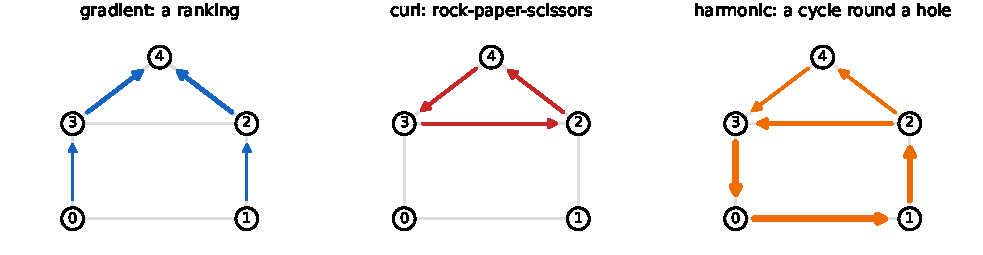
\includegraphics[width=\columnwidth]{figures/schematic.pdf}
\caption{The three Hodge components of one edge flow on a five-item
comparison graph (triangle 2--3--4 filled): a ranking, a local cycle, and a
cycle around the square hole. Arrow width is flow magnitude.}
\label{fig:schematic}
\end{figure}

That literature asks what a model \emph{can} represent. We ask what gradient
descent \emph{learns first}. The question has teeth. If a flexible preference
model fits the ranking long before it fits the cycles, then (i) the number of
training steps is an implicit prior on transitivity; (ii) early stopping acts
as a transitivity filter, discarding cyclic structure whether it is real or
noise; and (iii) since random label noise on a well-connected graph falls
almost entirely in cycle space, that filter should be most useful exactly when
annotators disagree. The neural tangent kernel \cite{jacot2018neural} is the
natural tool: in the linearised regime \cite{lee2019wide}, gradient descent
fits each eigen-direction of the kernel at a rate set by its eigenvalue, and
the infinite-width limit is a Gaussian process \cite{neal1996bayesian,
lee2018deep} --- here a GP preference model \cite{chu2005preference} with a
specific, computable kernel. What is missing is the kernel \emph{between
edges} and its relation to the Hodge subspaces.

We compute that kernel for three models, in closed form at infinite width and
empirically at finite width, and test four hypotheses: that the scalar
kernel is blind to cycles (H0); that the antisymmetric kernel is spectrally
ordered, gradient first (H1); that training follows that order (H2); and that
noise is cyclic and early stopping filters it (H3). We then test the whole
picture on \AreVotes\ human votes from Chatbot Arena (H4). H0--H2 hold
cleanly; parts of H1 and H3 do not, and we report where and why.

\section{Related work}
\label{sec:related}

\paragraph{Neural tangent kernels and spectral bias.} The NTK
\cite{jacot2018neural} describes gradient descent on wide networks as kernel
regression; wide networks evolve as their linearisation \cite{lee2019wide},
and their priors are Gaussian processes \cite{neal1996bayesian, lee2018deep}.
Directions with large kernel eigenvalues are learned first --- the spectral or
frequency bias \cite{rahaman2019spectral}. Output scaling moves a network
between this lazy regime and feature learning \cite{chizat2019lazy}. We use
all of these, but on a kernel defined over \emph{pairs} and decomposed by
graph topology rather than by frequency.

\paragraph{Hodge theory for rankings.} HodgeRank
\cite{jiang2011statistical} fits the gradient component by least squares and
reads the curl and harmonic residuals as measures of inconsistency; later work
uses it for crowdsourced ranking and Bayesian intransitive models
\cite{xu2018hodgerank}. No neural network or training dynamics is involved.

\paragraph{Intransitive preference models.} Bradley--Terry
\cite{bradley1952rank} underlies RLHF reward models \cite{ouyang2022training}.
GPM \cite{zhang2025beyond} embeds responses and scores pairs with a
skew-symmetric bilinear form; HRC \cite{hrc2026transitivity} decomposes
preferences into an explicit transitive scalar and a cyclic vector part. These
works establish expressivity and downstream gains; we study the learning
dynamics that any such model is subject to.

\paragraph{NTK for pairwise feedback.} Neural dueling bandits analyse
Bradley--Terry preference learning in the NTK regime to obtain confidence
bounds \cite{verma2024neural}; they do not decompose the kernel by Hodge
structure. The closest work is the Topological NTK \cite{krishnagopal2026topological},
which reports a ``topological spectral bias'' for message passing on edge
signals of simplicial complexes; it concerns graph neural networks on a fixed
complex, not preference models over item features, and does not address
Bradley--Terry losses, annotator noise or early stopping.

\section{Hodge decomposition of the edge NTK}
\label{sec:theory}

\paragraph{Comparison graphs.} Items $1..n$ with features $x_i \in
\mathbb{R}^d$; a graph with oriented edges $(i,j)$, $i<j$; an edge flow $y
\in \mathbb{R}^E$, $y_{ij}$ the preference of $j$ over $i$ (a log-odds). With
the gradient $B:\mathbb{R}^V\to\mathbb{R}^E$, $(Bs)_{ij}=s_j-s_i$, and the
curl $C:\mathbb{R}^E\to\mathbb{R}^T$ over triangles, the Hodge decomposition
is $\mathbb{R}^E = \operatorname{im}B \oplus \operatorname{im}C^\top \oplus
\ker(BB^\top + C^\top C)$, with orthogonal projectors $P_{\text{grad}},
P_{\text{curl}}, P_{\text{harm}}$ of ranks $|V|-1$ (connected graph), the
number of independent triangles, and the first Betti number.

\paragraph{Three models and their edge kernels.} A preference model predicts
$g_{ij}$. The \emph{scalar} model $g_{ij}=f(x_j)-f(x_i)$; the
\emph{antisymmetric} model $g_{ij} = h([x_i,x_j]) - h([x_j,x_i])$; GPM $g_{ij}
= e(x_i)^\top R\, e(x_j)$ with $R$ block-skew. Each is an MLP in the NTK
parameterisation. Under gradient descent with step $\eta$ on
$\tfrac{1}{2E}\sum(g-y)^2$ the training residual evolves, in the linearised
regime, as $r_{t+1} = (I-\tfrac{\eta}{E}\Theta_E)\,r_t$, where $\Theta_E$ is
the NTK between edges. For the scalar model $\Theta_E = B\,\Theta_V B^\top$
with $\Theta_V$ the ordinary NTK between items; for the antisymmetric model,
with $z=[x_i,x_j]$ and $\tilde z=[x_j,x_i]$,
\begin{equation}
\Theta_E(e,e') = K(z,z') - K(z,\tilde z') - K(\tilde z,z') + K(\tilde z,\tilde z'),
\end{equation}
$K$ the closed-form ReLU NTK \cite{jacot2018neural} on concatenated inputs.
We define the \emph{Hodge rate} of a component as the mean eigenvalue of
$\Theta_E$ on its subspace, $\kappa_c = \operatorname{tr}(P_c\Theta_E P_c)
/ \dim_c$ --- the expected Rayleigh quotient of a random flow in that
component, hence its expected learning speed.

\paragraph{Proposition 1 (the scalar kernel is blind to cycles).} For any
cyclic flow $y_c \in \ker B^\top$, $\Theta_E\,y_c = B\Theta_V B^\top y_c = 0$.
The cyclic residual of a scalar model therefore never changes under gradient
descent on the squared loss, at any width and in any regime: it is not merely
unrepresentable but invisible to the gradient. Numerically $|\kappa_{\text{cyc}}|
\le \SpeScalarCycMax$ across all graphs.

\paragraph{Why the antisymmetric kernel prefers rankings.} Split the kernel on
concatenated inputs into a part additive in its two halves and an interaction
part. The additive part yields, after antisymmetrisation, a term of the form
$B\,\tilde K\,B^\top$ --- the scalar structure again --- whose action on cycles
vanishes by Proposition 1, while on gradient flows it is amplified by the
number of edges that share each item. Cycles are therefore learned only
through the interaction part. This predicts (i) $\kappa_{\text{grad}} \gg
\kappa_{\text{cyc}}$, (ii) a ratio that grows with the mean degree of the
comparison graph, and (iii) no reason for curl and harmonic cycles to differ.

\paragraph{Lemma 2 (i.i.d.\ noise is mostly cyclic).} If $z \sim
\mathcal{N}(0,\sigma^2 I_E)$, rotational invariance makes $\|P_{\text{grad}}
z\|^2/\|z\|^2 \sim \text{Beta}(\tfrac{|V|-1}{2}, \tfrac{|E|-|V|+1}{2})$, with
mean $(|V|-1)/|E|$. On a complete graph that is $2/n$: almost all noise lives
where a transitive-first learner looks last.

\section{Spectrum and learning dynamics}
\label{sec:dynamics}

\begin{figure*}[t]
\centering
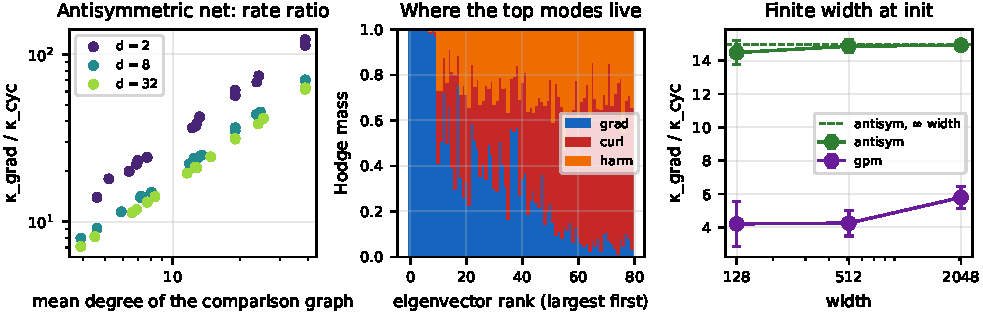
\includegraphics[width=\textwidth]{figures/spectrum.pdf}
\caption{Edge NTK of the antisymmetric network. Left: ratio of the mean kernel
eigenvalue on gradient flows to that on cyclic flows, over \SpeNGraphs\ random
comparison graphs (sizes 20 and 40, densities 0.15--1, depth 1 shown), against
the mean degree; colour is the feature dimension. Middle: Hodge composition of
the top 80 eigenvectors on a \SpeCanonN-item graph (\SpeCanonE\ edges;
gradient/curl/harmonic dimensions \SpeCanonGradDim/\SpeCanonCurlDim/\SpeCanonHarmDim).
Right: the same ratio for the empirical kernel at initialisation versus width,
with the infinite-width value dashed; GPM is shown for comparison.}
\label{fig:spectrum}
\end{figure*}

\paragraph{The spectrum is ordered.} Figure~\ref{fig:spectrum} confirms H1
for the gradient-versus-cycle split. In every one of the \SpeNGraphs\ graphs
the antisymmetric kernel's gradient rate exceeds its cyclic rate, by
\SpeRatioMin$\times$ on the sparsest graphs to \SpeRatioMax$\times$ on
complete ones (mean \SpeRatioSparse$\times$ at density 0.15,
\SpeRatioDense$\times$ at density 1), and the ratio grows with the mean
degree, as the additive-part argument predicts. Low feature dimension and
shallow networks sharpen it (\SpeRatioLowD$\times$ at $d=\SpeLowD$ versus
\SpeRatioHighD$\times$ at $d=\SpeHighD$; \SpeRatioDepthOne$\times$ at depth 1
versus \SpeRatioDepthTwo$\times$ at depth 2), since both enlarge the
interaction part of the kernel. The top ten eigenvectors carry
\SpeTopTenGradMass\% of their mass in gradient space. At finite width the
empirical kernel reproduces the analytic ratio already at width
\SpeEmpWLo\ (\SpeEmpAntisymWLo\ versus \SpeAnaRatioCanon), and the kernels agree
entrywise to \SpeEmpErrHi\% at width \SpeEmpWHi. GPM is ordered too but less
sharply (\SpeEmpGpmWLo--\SpeEmpGpmWHi$\times$): its bilinear form has no
additive part to amplify rankings.

\paragraph{Curl and harmonic are not ordered.} The second half of H1 fails.
The ratio of curl to harmonic rates ranges from \SpeCurlHarmMin\ to
\SpeCurlHarmMax\ with mean \SpeCurlHarmMean: the network does not distinguish
cycles around triangles from cycles around holes. This matches the argument
above --- both live only in the interaction part --- and it is where our
setting differs from the Topological NTK, whose message passing is built on
the Hodge Laplacian itself \cite{krishnagopal2026topological}.

\begin{figure*}[t]
\centering
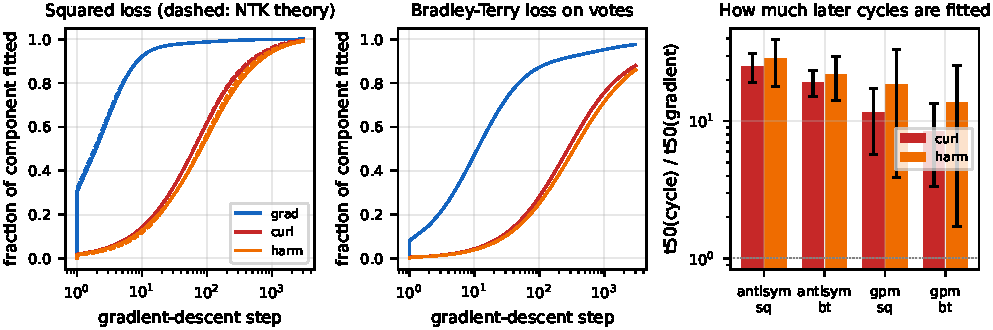
\includegraphics[width=\textwidth]{figures/dynamics.pdf}
\caption{Fraction of each Hodge component of the true flow fitted during
training (antisymmetric net, one seed). Left: squared loss, with the
linearised NTK prediction dashed. Middle: Bradley--Terry loss on 200 votes per
edge. Right: how many times later the cyclic components reach 50\% than the
gradient component, over seeds, for the antisymmetric net and GPM under both
losses.}
\label{fig:dynamics}
\end{figure*}

\paragraph{Training follows the spectrum.} On a synthetic task
(\TaskN\ items, $d=\TaskD$, density \TaskDens; the true preference combines a
smooth utility and a skew interaction, giving
\TaskFracGrad/\TaskFracCurl/\TaskFracHarm\% gradient/curl/harmonic energy),
Figure~\ref{fig:dynamics} shows H2. The antisymmetric network fits the
ranking in a handful of steps and the cycles \DynAntisymSqCurl$\times$ (curl)
and \DynAntisymSqHarm$\times$ (harmonic) later under the squared loss, and
\DynAntisymBtCurl$\times$ and \DynAntisymBtHarm$\times$ later under the
Bradley--Terry loss on votes; GPM shows the same order with a smaller gap
(\DynGpmSqCurl$\times$ and \DynGpmSqHarm$\times$). The order held in
\DynOrderOk\ of \DynOrderTotal\ runs. Under the squared loss the linearised
NTK prediction tracks the network's per-component fit to within \DynLinDev\
at every step --- the dynamics \emph{is} the spectrum. The scalar model fits
the ranking just as fast and never moves on cycles (final curl fit
$\le\DynScalarCurlFinal$), which costs it on held-out pairs: \DynHoScalar\
sign accuracy versus \DynHoAntisym\ (antisymmetric) and \DynHoGpm\ (GPM),
because the true preferences are partly cyclic.

\begin{figure*}[t]
\centering
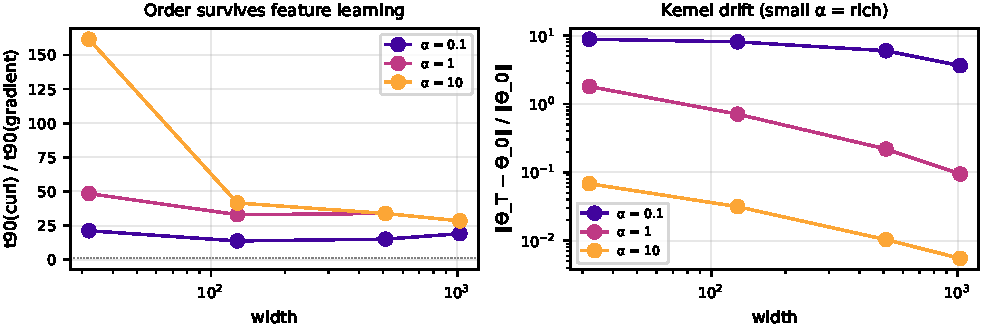
\includegraphics[width=0.8\textwidth]{figures/width.pdf}
\caption{Antisymmetric net across width and output scale $\alpha$ (small
$\alpha$ = rich, feature learning). Left: how many times later curl reaches
90\% than the gradient part. Right: relative change of the empirical kernel
over training.}
\label{fig:width}
\end{figure*}

\paragraph{Feature learning narrows the gap but keeps the order.}
Figure~\ref{fig:width} moves the network out of the kernel regime. With
$\alpha=\WidAlphaLazy$ the kernel barely moves (relative drift
\WidDriftLazy) and curl reaches 90\% \WidRatioLazy$\times$ after the ranking;
with $\alpha=\WidAlphaRich$ the kernel changes by a factor of
\WidDriftRich\ and the gap shrinks to \WidRatioRich$\times$, because the
evolving kernel becomes less ordered (final rate ratio \WidKRatioRich\ versus
\WidKRatioLazy). The order held in all \WidOrderOk\ of \WidRuns\ runs across
widths \WidMin--\WidMax. Feature learning here also generalises slightly
better (held-out \WidAccRich\ versus \WidAccLazy): it learns the cycles sooner.

\section{Noise and early stopping}
\label{sec:noise}

\begin{figure*}[t]
\centering
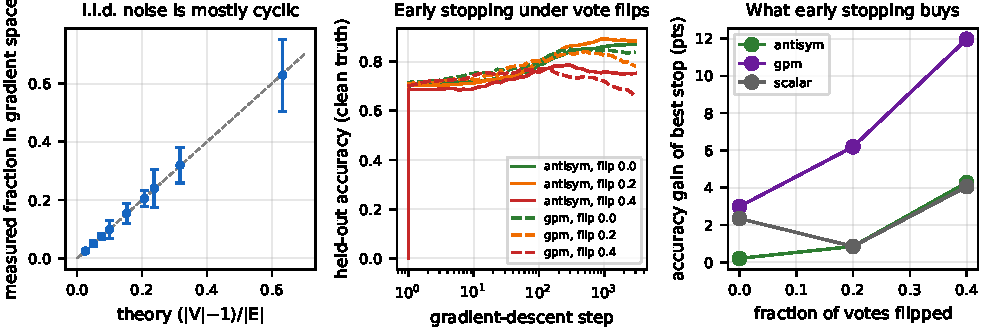
\includegraphics[width=\textwidth]{figures/noise.pdf}
\caption{Left: fraction of i.i.d.\ Gaussian edge noise in gradient space
against Lemma 2, over \NoiFracCases\ graphs (error bars: one standard
deviation over draws). Middle: held-out sign accuracy against the clean truth
during training with 0, 20 and 40\% of votes flipped (mean of seeds). Right:
accuracy gained by stopping at the best step instead of training to the end,
by model and flip rate.}
\label{fig:noise}
\end{figure*}

\paragraph{Random noise is cyclic --- annotator flips are not.} Lemma 2 holds
to within \NoiFracMaxDev\ in all \NoiFracCases\ graphs
(Figure~\ref{fig:noise}, left); on the densest graph (\NoiFracDenseN\ items,
\NoiFracDenseE\ edges) only \NoiFracDense\ of the noise is transitive. On the
synthetic task the prediction is \NoiTheoryTask\ and Gaussian noise puts
\NoiGaussGradFrac\ there. Vote flips behave differently: \NoiFlipGradFrac\ of
the resulting perturbation lies in gradient space. A flip rate $\epsilon$
pulls every win probability toward one half, so its main effect is to
\emph{shrink} the true flow --- which is mostly transitive --- rather than to
add independent noise. The clean ``noise is cyclic'' story therefore applies
to measurement noise, not to annotators who randomly disagree.

\paragraph{Early stopping helps, but not where the ranking is fitted.} Our
predicted stopping time $t^\star$, the step at which the linearised gradient
component is 95\% fitted, is too early: held-out accuracy there is
\NoiAntisymAtTstarClean\ against \NoiAntisymBestClean\ at the best step for
the antisymmetric net, because stopping when the ranking is learned also
discards the \emph{true} cycles. Early stopping still earns its keep, and more
so as noise grows (Figure~\ref{fig:noise}, middle and right). The best step
moves earlier with noise (from \NoiAntisymStepBestClean\ to
\NoiAntisymStepBestFlipFour\ steps for the antisymmetric net, \NoiGpmStepBestClean\
to \NoiGpmStepBestFlipFour\ for GPM). At 40\% flipped votes it recovers
\NoiAntisymGainFlipFour\ accuracy points for the antisymmetric net
(\NoiAntisymFinalFlipFour\ $\to$ \NoiAntisymBestFlipFour) and
\NoiGpmGainFlipFour\ for GPM (\NoiGpmFinalFlipFour\ $\to$ \NoiGpmBestFlipFour).
The scalar model, which cannot overfit cycles at all, gains
\NoiScalarGainFlipFour. The right stopping time lies \emph{between} the
gradient and cycle time scales, and where it falls depends on how much of the
cyclic content is signal. The spectrum tells us the two time scales; it cannot
by itself tell us that ratio.

\section{Chatbot Arena}
\label{sec:arena}

\begin{figure*}[t]
\centering
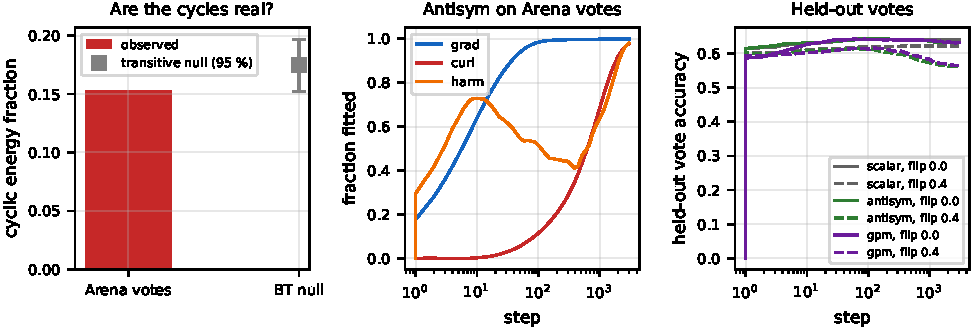
\includegraphics[width=\textwidth]{figures/arena.pdf}
\caption{Chatbot Arena, \AreItems\ models, \AreEdges\ model pairs with at
least \AreMinVotes\ votes. Left: cyclic energy of the observed log-odds flow
against a perfectly transitive Bradley--Terry null with the same counts
(median and 95\% interval). Middle: per-component fit of the antisymmetric
net under the Bradley--Terry loss. Right: held-out vote accuracy during
training, clean and with 40\% of training votes flipped (mean of seeds).}
\label{fig:arena}
\end{figure*}

We take \AreVotes\ human votes between \AreItems\ LLMs from the public Chatbot
Arena release \cite{chiang2024chatbot}, keep the \AreEdges\ model pairs with
at least \AreMinVotes\ votes, count ties as half a win, and hold out 20\% of
votes per pair (\AreHoN\ decisive held-out votes). Items have no features, so
each network sees a one-hot model identity.

\paragraph{The cycles in Arena are sampling noise.} The observed flow has
\AreFracGrad\% gradient and \AreCyc\% cyclic energy (the graph has
\AreDimCurl\ triangle dimensions and only \AreDimHarm\ harmonic ones). Is
that intransitivity? We simulate votes from the best transitive fit with the
\emph{same} per-pair counts: finite samples alone produce \AreNullCyc\% cyclic
energy (95\% interval \AreNullCycLo--\AreNullCycHi\%). The observed value sits
\emph{below} the null ($p=\AreP$ for cycles at least as strong). At the level
of models, Arena preferences show no intransitivity beyond what counting noise
creates --- which is Lemma 2 at work on real data.

\paragraph{The same order, and what it implies.} On these votes the
antisymmetric kernel ranks gradient over cycles by \AreAntisymRatio$\times$
(GPM \AreGpmRatio$\times$), and training fits the ranking by step
\AreAntisymTGrad\ and the cycles only around step \AreAntisymTCurl\
(Figure~\ref{fig:arena}, middle). Since the cycles are noise, the flexible
models' late phase is pure overfitting. Trained to the end, the scalar model is
the best held-out predictor (log-loss \AreScalarLLClean, accuracy
\AreScalarAccClean, matching HodgeRank's \AreHodgeLL\ and \AreHodgeAcc),
ahead of the antisymmetric net (\AreAntisymLLClean) and GPM (\AreGpmLLClean).
With 40\% of training votes flipped the gap widens (accuracy
\AreScalarAccFlipFour\ versus \AreAntisymAccFlipFour\ and \AreGpmAccFlipFour),
and early stopping recovers most of it (best
\AreAntisymBestFlipFour\ and \AreGpmBestFlipFour). Stopped early, a cyclic
model is a scalar model.

\section{Limitations and conclusion}
\label{sec:conclusion}

\paragraph{Limitations.} The kernel analysis is exact at infinite width and
for the squared loss; the Bradley--Terry and feature-learning results are
empirical. Our networks are small MLPs on low-dimensional features, not reward
models on top of a language model, where the ``items'' are responses with rich
embeddings and each response appears in few comparisons --- a sparse regime in
which our ratio is smallest. The synthetic truth mixes one utility with one
skew interaction; other cyclic structures could be learned at different
speeds. The Arena analysis is at model level, so it says nothing about
prompt-level intransitivity, where genuine cycles are more plausible, and
held-out votes are split within pairs, so they test fitting of observed pairs
more than generalisation to unseen ones. The NTK stopping rule we proposed
failed; a rule that estimates the signal fraction in cycle space, for example
with the transitive null of Section~\ref{sec:arena}, is the natural
replacement. The full-scale configuration widens every sweep.

\paragraph{Conclusion.} Gradient descent learns preferences in a fixed order:
the ranking first, the cycles much later. For a scalar reward model the
cycles are not merely unrepresentable but invisible to the gradient. For an
antisymmetric network the edge NTK puts transitive flows 4 to over 100 times
higher in the spectrum than cyclic ones, more so on denser comparison graphs,
and training follows that ordering, closely in the lazy regime and robustly
beyond it. Local and global cycles, by contrast, are learned at the same
rate. The ordering turns training time into a knob on transitivity. It
explains why early stopping helps cyclic preference models most when votes are
noisy. It also cautions against reading learned cycles as signal: in Chatbot
Arena, the cycles a flexible model eventually learns are sampling noise,
fitted last.


\FloatBarrier
\bibliographystyle{plain}
\bibliography{references}

\end{document}
